%%%%%%%%%%%%%%%%%%%%%%%%%%%%%%%%%%%%%%%%%
% Short Sectioned Assignment LaTeX Template Version 1.0 (5/5/12)
% This template has been downloaded from: http://www.LaTeXTemplates.com
% Original author:  Frits Wenneker (http://www.howtotex.com)
% License: CC BY-NC-SA 3.0 (http://creativecommons.org/licenses/by-nc-sa/3.0/)
%%%%%%%%%%%%%%%%%%%%%%%%%%%%%%%%%%%%%%%%%

%----------------------------------------------------------------------------------------
%	PACKAGES AND OTHER DOCUMENT CONFIGURATIONS
%----------------------------------------------------------------------------------------

\documentclass[paper=a4, fontsize=11pt]{scrartcl} % A4 paper and 11pt font size

% ---- Entrada y salida de texto -----

\usepackage[T1]{fontenc} % Use 8-bit encoding that has 256 glyphs
\usepackage[utf8]{inputenc}
%\usepackage{fourier} % Use the Adobe Utopia font for the document - comment this line to return to the LaTeX default

% ---- Idioma --------

\usepackage[spanish, es-tabla]{babel} % Selecciona el español para palabras introducidas automáticamente, p.ej. "septiembre" en la fecha y especifica que se use la palabra Tabla en vez de Cuadro

% ---- Otros paquetes ----

\usepackage{url} % ,href} %para incluir URLs e hipervínculos dentro del texto (aunque hay que instalar href)
\usepackage{amsmath,amsfonts,amsthm} % Math packages
%\usepackage{graphics,graphicx, floatrow} %para incluir imágenes y notas en las imágenes
\usepackage{graphics,graphicx, float} %para incluir imágenes y colocarlas
% Para hacer cuadros
\usepackage{tcolorbox}
% Para hacer uso de párrafos
\usepackage{parskip}
\usepackage{hyperref}
\usepackage{vmargin}
\setpapersize{A4}
\setmargins{2.5cm}       % margen izquierdo
{1.5cm}                        % margen superior
{16.5cm}                      % anchura del texto
{23.42cm}                    % altura del texto
{10pt}                           % altura de los encabezados
{1cm}                           % espacio entre el texto y los encabezados
{0pt}                             % altura del pie de página
{2cm}                           % espacio entre el texto y el pie de página
% Para hacer tablas comlejas
%\usepackage{multirow}
%\usepackage{threeparttable}

%\usepackage{sectsty} % Allows customizing section commands
%\allsectionsfont{\centering \normalfont\scshape} % Make all sections centered, the default font and small caps

\usepackage{fancyhdr} % Custom headers and footers
\pagestyle{fancyplain} % Makes all pages in the document conform to the custom headers and footers
\fancyhead{} % No page header - if you want one, create it in the same way as the footers below
\fancyfoot[L]{Mario López González 3ºB} % Empty left footer
\fancyfoot[C]{} % Empty center footer
\fancyfoot[R]{\thepage} % Page numbering for right footer
\renewcommand{\headrulewidth}{0pt} % Remove header underlines
\renewcommand{\footrulewidth}{0pt} % Remove footer underlines
\setlength{\headheight}{13.6pt} % Customize the height of the header

\numberwithin{equation}{section} % Number equations within sections (i.e. 1.1, 1.2, 2.1, 2.2 instead of 1, 2, 3, 4)
\numberwithin{figure}{section} % Number figures within sections (i.e. 1.1, 1.2, 2.1, 2.2 instead of 1, 2, 3, 4)
\numberwithin{table}{section} % Number tables within sections (i.e. 1.1, 1.2, 2.1, 2.2 instead of 1, 2, 3, 4)

\setlength\parindent{0pt} % Removes all indentation from paragraphs - comment this line for an assignment with lots of text

\newcommand{\horrule}[1]{\rule{\linewidth}{#1}} % Create horizontal rule command with 1 argument of height


\title{	
\normalfont \normalsize 
\textsc{\textbf{Ingeniería de Servidores (2021-2022)} \\ Grado en Ingeniería Informática \\ Universidad de Granada} \\ [25pt] % Your university, school and/or department name(s)
\horrule{0.5pt} \\[0.4cm] % Thin top horizontal rule
\huge Memoria Práctica 4 \\ % The assignment title
\horrule{2pt} \\[0.5cm] % Thick bottom horizontal rule
}

\author{Mario López González} % Nombre y apellidos

\date{\normalsize\today} % Incluye la fecha actual

%----------------------------------------------------------------------------------------
% DOCUMENTO
%----------------------------------------------------------------------------------------

\begin{document}

\maketitle % Muestra el Título

\begin{figure}[H]
    \centering
    
\includegraphics[scale=0.175]{images/server.jpg}
    \label{fig:server}
\end{figure}

\newpage %inserta un salto de página

\tableofcontents % para generar el índice de contenidos
\listoffigures % para generar el índice de imágenes

%%%%%%%%%%%%%%%%%%%%%%%%%%%%%%%%%%%%%%%%%%%%%%%%% 
% Apartado para la instalación en Ubuntu Server %
%%%%%%%%%%%%%%%%%%%%%%%%%%%%%%%%%%%%%%%%%%%%%%%%%
\newpage
\section{Phoronix}
\subsection{Instalación}
\subsubsection{Ubuntu Server}
Para instalar Phoronix en Ubuntu Server lo primero que tenemos que hacer es descargarnos la versión actual más estable con el siguiente comando:
\begin{tcolorbox}[colback=black!10, halign=left]
    \$ wget http://phoronix-test-suite.com/releases/repo/pts.debian/files/phoronix-test-suite\_8.6.0\_all.deb
\end{tcolorbox}

Una vez lo hemos descargado, procedemos a instalarlo con el comando dpkg:
\begin{tcolorbox}[colback=black!10, halign=left]
    \$ sudo dpkg -i phoronix-test-suite\_8.6.0\_all.deb
\end{tcolorbox}

Por último, solucionamos cualquier problema que pueda existir con las dependencias con el siguiente comando:
\begin{tcolorbox}[colback=black!10, halign=left]
    \$ sudo apt -f install
\end{tcolorbox}

\subsubsection{CentOS}
Para instalar Phoronix en CentOS lo primero que tenemos que hacer es descargarnos e instalar las dependencias necesarias para su ejecución:
\begin{tcolorbox}[colback=black!10, halign=left]
    \# sudo yum install wget php-cli php-xml bzip2
\end{tcolorbox}

Una vez hemos instalado las dependencias procedemos descargar la versión actual más estable para CentOS:
\begin{tcolorbox}[colback=black!10, halign=left]
    \# wget https://phoronix-test-suite.com/releases/phoronix-test-suite-8.6.0.tar.gz
\end{tcolorbox}

Cuando se hayan descargado los paquetes los extraemos:
\begin{tcolorbox}[colback=black!10, halign=left]
    \# tar xvfz phoronix-test-suite-8.4.1.tar.gz
\end{tcolorbox}

Por último, instalamos el fichero \textbf{\emph{install-sh}} que se encuentra dentro de la carpeta que acabamos de extraer:
\begin{tcolorbox}[colback=black!10, halign=left]
    \# sudo ./install-sh
\end{tcolorbox}

\subsection{Benchmarks}
\subsubsection{RAMspeed SMP}
Este benchmark se encarga de medir el rendimiento de los módulos RAM realizando una serie de operaciones que le indica el usuario. En mi caso,
he decidido ejecutar el test con la operación \emph{copy} con datos de tipo entero.

La ejecución de los test se hace con el comando "phoronix-test-suite run <benchmark>". En este caso la ejecución del benchmark sería de la siguiente manera:
\begin{tcolorbox}[colback=black!10, halign=left]
    \# phoronix-test-suite run ramspeed
\end{tcolorbox}

\begin{figure}[H]
    \centering
    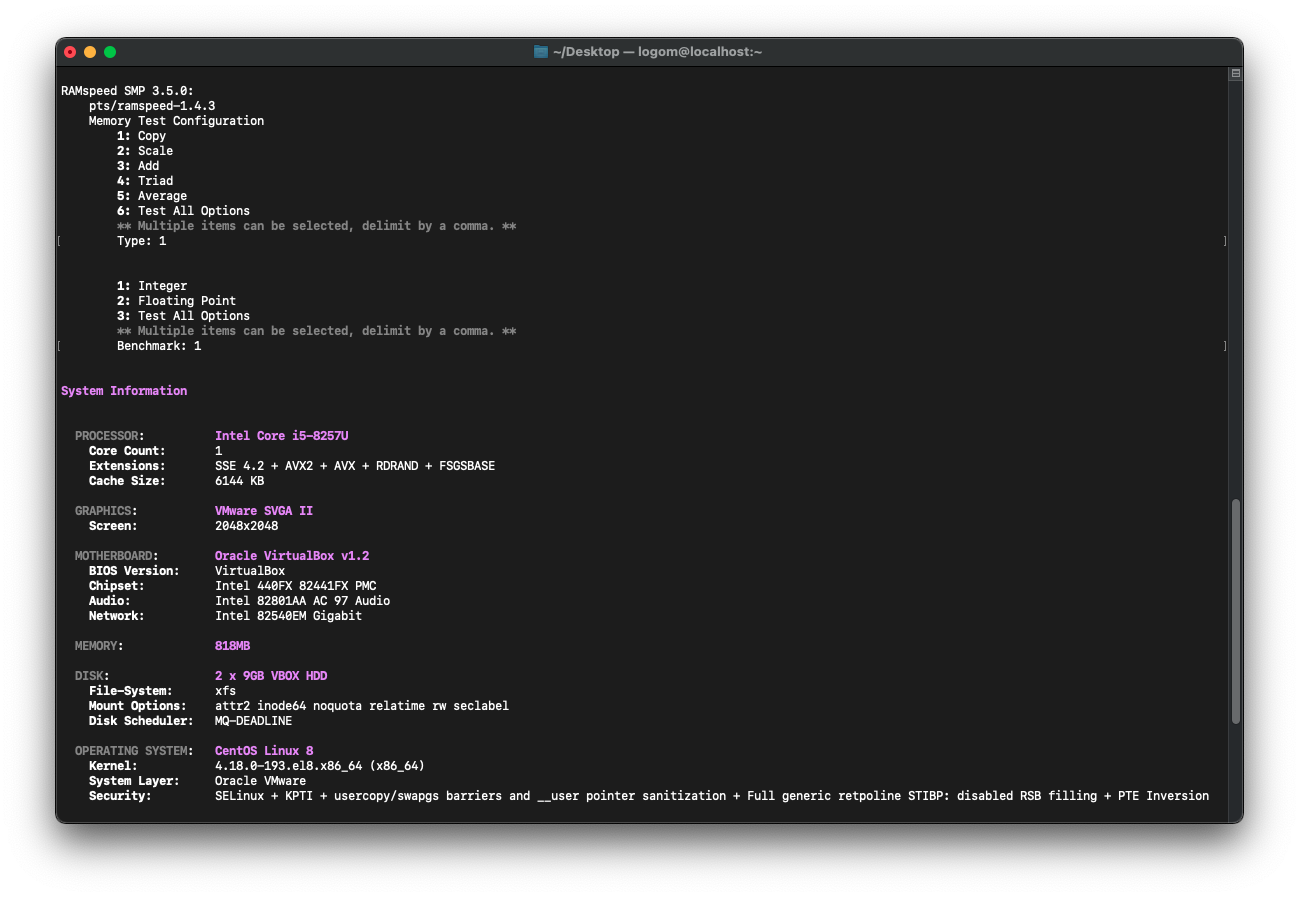
\includegraphics[scale=0.36]{images/ramspeed_parametros.png}
    \caption{Parámetros para RAMspeed SMP}
    \label{fig:ramspeed_parametros}
\end{figure}

La imagen anterior contiene información sobre el hardware de nuestra máquina como puede ser la CPU o la cantidad de memoria principal instalada. Dicha información se muestra de
manera automática al ejecutar el test.

El test se ha ejecutado tanto en Ubuntu Server como en CentOS. En Ubuntu el tiempo estimado del test ha sido 22 minutos, mientras que en CentOS ha sido de 5 minutos. Por defecto, 
está programado para ejecutar tres test, aunque puede considerar conveniente realizar más test para una mayor precisión en sus cálculos. En mi caso, en CentOS ha realizado el
número de test predeterminados, sin embargo, en Ubuntu ha ocurrido lo contrario, en lugar de realizar tres test ha hecho seis. Debido al número de test realizados en Ubuntu cobra
sentido la diferencia de tiempo entre ambos test.

\begin{figure}[H]
    \centering
    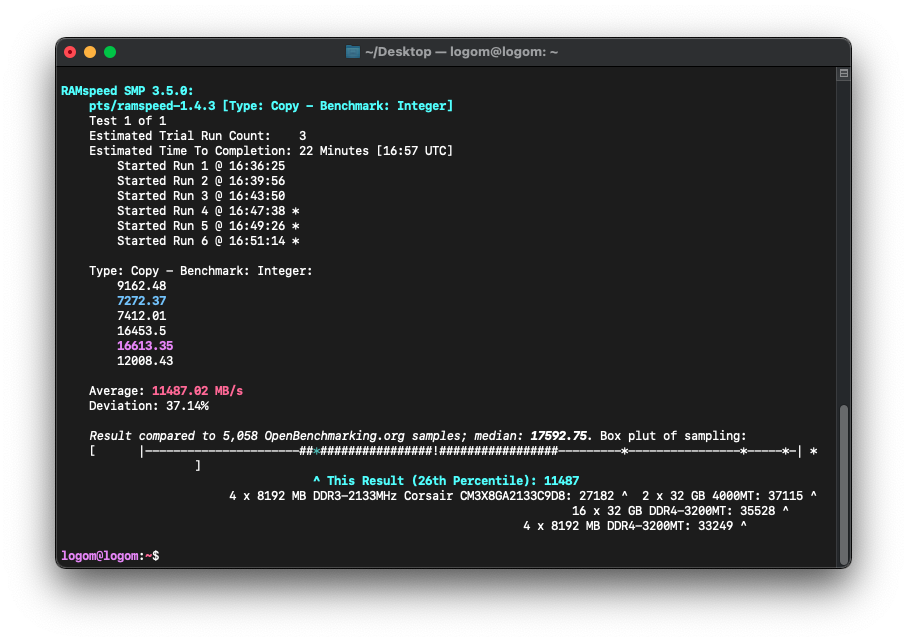
\includegraphics[scale=0.5]{images/ramspeed_ubuntu.png}
    \caption{Ejecución de RAMspeed SMP en Ubuntu Server}
    \label{fig:ramspeed_ubuntu}
\end{figure}

\begin{figure}[H]
    \centering
    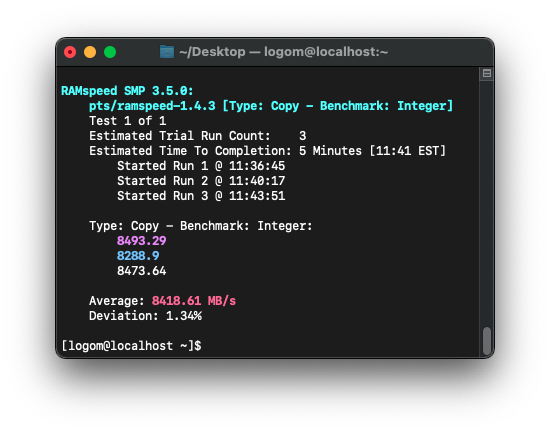
\includegraphics[scale=0.6]{images/ramspeed_centos.png}
    \caption{Ejecución de RAMspeed SMP en CentOS}
    \label{fig:ramspeed_centos}
\end{figure}

He calculado el coeficiente de variación ($cv$) de ambos test, $cv = (deviation / 100) / average$, concluyendo en que el test realizado en CentOS es más fiable que el realizado en Ubuntu.

La velocidad de los test deberían ser similares ya que se están ejecutando sobre el mismo hardware por lo que tomaré como velocidad de referencia la calculada en el test de CentOS.

\subsubsection{Sudokut}
Este benchmark mide el rendimiento de la CPU. Para ello, mide el tiempo que tarda el procesador en resolver 100 sudokus.

La ejecución de este test no arroja resultados tan dispares como en el test anterior. En este caso, la diferencia es minima, de unas pocas milésimas.

\begin{figure}[H]
    \centering
    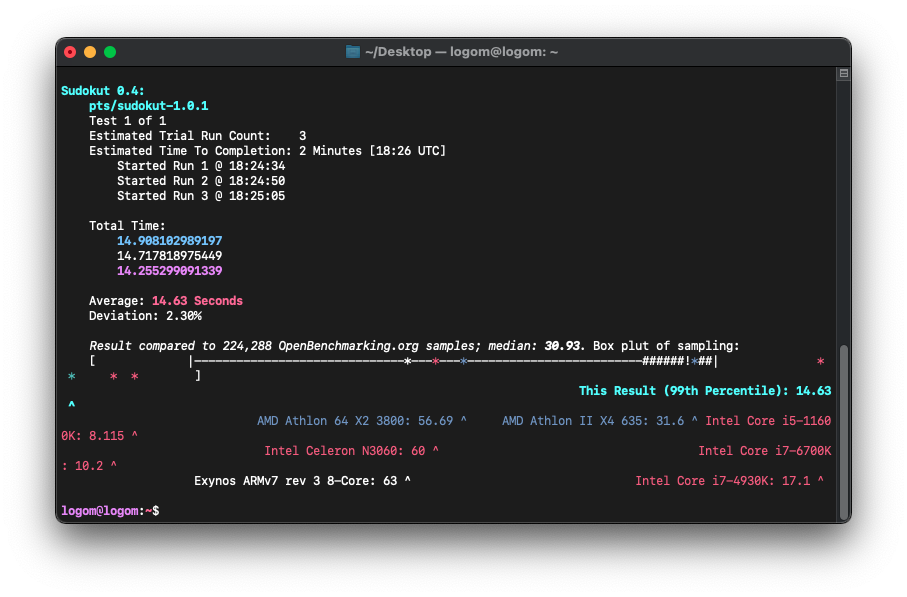
\includegraphics[scale=0.5]{images/sudokut_ubuntu.png}
    \caption{Ejecución de Sudokut en Ubuntu Server}
    \label{fig:sudokut_ubuntu}
\end{figure}

\begin{figure}[H]
    \centering
    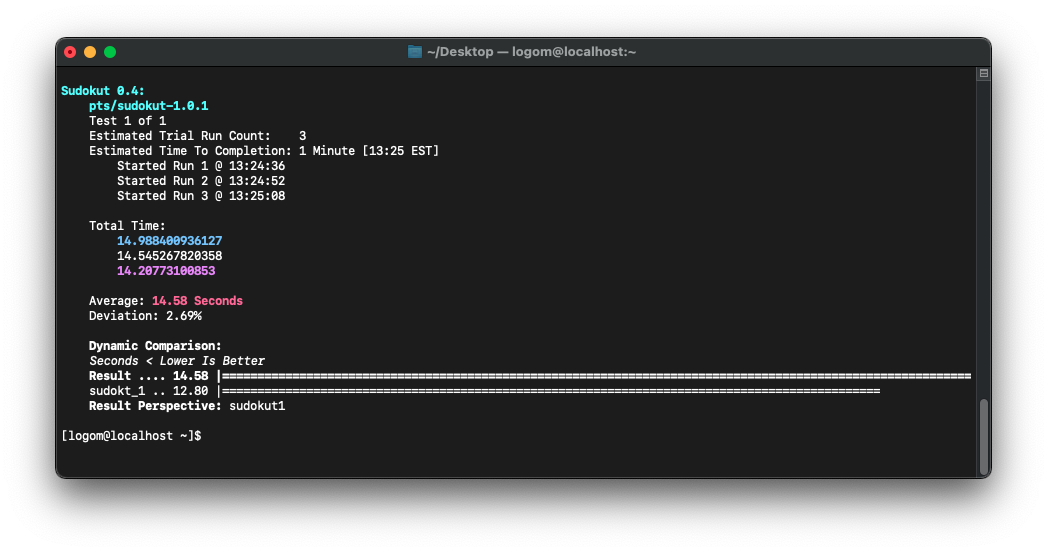
\includegraphics[scale=0.4]{images/sudokut_centos.png}
    \caption{Ejecución de Sudokut en CentOS}
    \label{fig:sudokut_centos}
\end{figure}

Como se puede observar en las imágenes anteriores, se han realizado el mismo número de tests y con la misma estimación de tiempo. Sin embargo, tras calcular los 
coeficientes de variación y su correspondiente comparativa, concluyo en que los resultados obtenidos en el test de Ubuntu son más fiables por lo que tomaré su
tiempo como valor de referencia.

\begin{thebibliography}{0}
    \bibitem{} \href{}{}
\end{thebibliography}

\end{document}
